\documentclass[conference]{IEEEtran}
\IEEEoverridecommandlockouts
\usepackage{cite}
\usepackage{amsmath,amssymb,amsfonts}
\usepackage{algorithm}
\usepackage{algorithmic}
\usepackage{graphicx}
\usepackage{textcomp}
\usepackage{xcolor}
\usepackage{placeins}
\usepackage{booktabs}
\def\BibTeX{{\rm B\kern-.05em{\sc i\kern-.025em b}\kern-.08em
    T\kern-.1667em\lower.7ex\hbox{E}\kern-.125emX}}

\begin{document}

\title{A Game Theory Based Collusion Aware Auction Framework for Agentic Compute Markets}

\author{
\IEEEauthorblockN{1\textsuperscript{st} Om Ashok Nalage}
\IEEEauthorblockA{\textit{Department of Computer Science and Engineering} \\
\textit{Visvesvaraya National Institute of Technology (VNIT)}\\
Nagpur, India \\
omashoknalage@gmail.com}
\and
\IEEEauthorblockN{2\textsuperscript{nd} Prabhat Kumar Prince}
\IEEEauthorblockA{\textit{Department of Computer Science and Engineering} \\
\textit{Visvesvaraya National Institute of Technology (VNIT)}\\
Nagpur, India \\
prabhatprince321@gmail.com}
\and
\IEEEauthorblockN{3\textsuperscript{rd} Rajat Samarth}
\IEEEauthorblockA{\textit{Department of Computer Science and Engineering} \\
\textit{Visvesvaraya National Institute of Technology (VNIT)}\\
Nagpur, India \\
rsamarth22@gmail.com}
\and
\IEEEauthorblockN{4\textsuperscript{th} Sakshi Pore}
\IEEEauthorblockA{\textit{Department of Computer Science and Engineering} \\
\textit{Visvesvaraya National Institute of Technology (VNIT)}\\
Nagpur, India \\
poresakshi344@gmail.com}
}

\maketitle

\begin{abstract}
This paper presents the Python simulation implemented in this project for comparing the Vickrey method, implemented as a reserve-constrained second-price auction, against an improved collusion-aware mechanism. The implementation is centered in \texttt{main.py}. It loads GPU specification data from \texttt{datasets/gpu\_specs\_v7.csv}, normalizes hardware columns, samples generated agents, simulates honest and collusive bidding behavior, extracts bid-distribution features, clears bids through a Vickrey-style second-price auction, and exports comparison graphs to the \texttt{graphs/} directory. The Vickrey method clears raw bids using the second-price rule without monitoring, historical memory, or bid enforcement. The improved mechanism keeps the same settlement rule but adds round-level feature extraction, online collusion-risk scoring with logistic regression, and history-aware bid adjustment before clearing. This design keeps the auction rule fixed while changing only the pre-clearing enforcement layer, so the Vickrey and improved results remain directly comparable. The simulation uses 1500 agents, 200 rounds per trial, and 20 deterministic seeded trials. It reports payment, seller profit, welfare proxy, and detector metrics. Seller profit is defined in the code as payment minus reserve floor, which makes the seller-side interpretation clearer than payment alone. All reported numerical values are produced by running the simulator: result tuples are appended during auction clearing, trial-level means are computed from those tuples, detector scores are computed from stored feature-label arrays, and the included comparison graphs are generated by the project plotting functions. In the latest run, the improved mechanism increases average payment from $3.8863$ to $4.6616$, average seller profit from $0.4352$ to $1.1649$, and average welfare proxy from $3.8909$ to $4.6664$. These correspond to gains of $19.95\%$, $167.68\%$, and $19.93\%$, respectively. Detector evaluation reports accuracy $0.9000$, ROC-AUC $0.9132$, precision $0.8941$, recall $0.9038$, FPR $0.1019$, and FNR $0.0962$ as 20-trial means. The project dataset used in the run contains 3056 source rows and 2823 merged GPU rows after filtering and deduplication, with missing release-price values handled by the fallback value path implemented in the code. The paper describes only the implemented simulation components, generated metrics, algorithms, and comparison graphs from the project.
\end{abstract}

\begin{IEEEkeywords}
game theory, Vickrey auction, second-price auction, collusion detection, agentic markets, compute marketplace, adaptive enforcement, seller profit
\end{IEEEkeywords}

\section{Introduction}
This project implements a repeated auction simulation using GPU-related input data, generated bidding agents, collusive bidding behavior, a reserve-constrained second-price auction, and a machine-learning-based improved path. The simulation compares two mechanisms under the same codebase: a Vickrey auction path and an improved path with bid adjustment.

The project is evaluated from the seller side using payment and seller profit. Payment is the second-price auction payment. Seller profit is computed as payment minus reserve floor for each cleared round. The project also reports a welfare proxy, implemented as the winning cleared bid.

The project compares two mechanisms. The Vickrey method is a reserve-constrained second-price auction. It takes raw bids, removes bids below a reserve floor, selects the highest valid bid as the winner, and charges the second-highest valid bid. The improved mechanism uses the same auction clearing rule, but adds an enforcement layer before clearing. It extracts round-level bid-pattern features, estimates collusion risk from previous rounds only, and adjusts bids using a history-aware rule scaled by the estimated risk.

The main purpose of the simulation is comparative: it measures whether the improved mechanism produces better reported outcomes than the Vickrey method in this implemented stochastic setting.

\subsection{Contributions}
This paper makes four implementation-centered contributions. First, it formalizes the Vickrey method auction mechanism and the improved collusion-aware mechanism in comparable notation. Second, it provides separate algorithms for the Vickrey and improved systems. Third, it defines seller profit as payment minus reserve floor. Fourth, it presents the comparison graphs generated by the project.

\subsection{Organization}
Section II lists background references for the components used by the project. Section III describes the project files and execution scope. Section IV defines the system model. Section V gives the metric definitions. Section VI provides the Vickrey method algorithm, and Section VII provides the improved algorithm. Section VIII describes simulation data, parameters, and metrics. Section IX reports numerical results. Section X presents comparison graphs. Section XI summarizes seller-side results. Section XII concludes the paper.

\section{Related Work}
The project uses a Vickrey-style second-price payment rule, where the highest valid bidder wins and the payment is the second-highest valid bid \cite{b1}. Standard auction references provide the background for this payment-rule family and auction notation \cite{b4,b5,b6,b7,b8}. The project uses scikit-learn models for detection and evaluation \cite{b2}. The offline detector uses a Random Forest classifier \cite{b9}, while the online improved path uses logistic regression \cite{b10}. The detector output is evaluated with accuracy, ROC-AUC, precision, recall, false-positive rate, and false-negative rate \cite{b3}. Bid-rigging detection literature is cited only as background for why bid-pattern monitoring is relevant to auction simulations \cite{b11}.

\section{Project Files and Execution Scope}
The reported experiment is generated by running \texttt{python3 main.py}. The file \texttt{main.py} contains the data loading, agent generation, feature extraction, detector definitions, auction implementation, bid adjustment, marketplace simulation, trial aggregation, and plotting functions used for the reported results. Other Python files are present in the repository, but the reported run and graph generation come from \texttt{main.py}.

\begin{table*}[htbp]
\caption{Project files used or generated by the reported run}
\label{tab:filemap}
\centering
\begin{tabular}{ll}
\toprule
\textbf{File or directory} & \textbf{Project role} \\
\midrule
\texttt{main.py} & Main executable simulation script \\
\texttt{datasets/gpu\_specs\_v7.csv} & Dataset loaded by \texttt{DATASET\_PATH} \\
\texttt{graphs/} & Output directory for generated figures \\
\texttt{comparison\_payments.png} & Vickrey method vs improved payment graph \\
\texttt{comparison\_welfare.png} & Vickrey method vs improved welfare graph \\
\texttt{comparison\_seller\_profit.png} & Vickrey method vs improved seller-profit graph \\
\texttt{seller\_profit\_summary.png} & Aggregate seller-profit bar graph \\
\texttt{paper/ieee\_paper\_conference.tex} & Conference paper source \\
\texttt{paper/ieee\_paper\_conference.pdf} & Compiled conference paper \\
\bottomrule
\end{tabular}
\end{table*}

\begin{table}[htbp]
\caption{Main implementation components in \texttt{main.py}}
\label{tab:codemap}
\centering
\begin{tabular}{ll}
\toprule
\textbf{Component} & \textbf{Implemented role} \\
\midrule
\texttt{load\_hardware\_data} & Reads and filters GPU rows \\
\texttt{generate\_agents} & Samples 1500 generated agents \\
\texttt{extract\_features} & Computes six bid-pattern features \\
\texttt{CollusionDetector} & Random Forest detector for evaluation \\
\texttt{Oracle} & Draws reserve floor values \\
\texttt{VCGAuction} & Clears valid bids by second price \\
\texttt{BidAdjuster} & Adjusts bids in improved path \\
\texttt{Marketplace} & Runs Vickrey method or improved simulation \\
\texttt{evaluate\_ml} & Reports detector metrics \\
\texttt{plot\_comparison} & Writes comparison graphs \\
\texttt{summarize\_trials} & Prints multi-trial summary \\
\bottomrule
\end{tabular}
\end{table}

The script sets \texttt{DEFAULT\_AGENT\_COUNT} to 1500, \texttt{DEFAULT\_ROUNDS} to 200, and \texttt{DEFAULT\_TRIALS} to 20. It sets \texttt{BASE\_SEED} to 42. Each trial creates a NumPy random generator using \texttt{BASE\_SEED + trial\_idx}. The Vickrey and improved marketplaces are both run inside each trial loop, and their results are stored in trial-level dictionaries before multi-trial aggregation.

\subsection{Marketplace State Kept During a Run}
The \texttt{Marketplace} class stores the values used for reporting and detector evaluation. The list \texttt{results} stores only cleared auction rounds. Each stored result is a tuple containing payment, welfare proxy, and seller profit. Payment and welfare are returned by \texttt{VCGAuction.run}; seller profit is then computed in \texttt{Marketplace.simulate} as payment minus the reserve floor, with a lower bound of zero. This means the paper's seller-profit values come from the clearing event and the actual reserve floor drawn in that round.

The simulator also stores \texttt{features} and \texttt{labels}. These are appended every round after raw bids are generated and the collusion label is created. The improved mechanism uses separate enforcement buffers, \texttt{\_enforce\_X} and \texttt{\_enforce\_y}, for online scoring. Those buffers are updated only after the current round has been scored and cleared. Therefore, the online score for a round is based on previous feature-label pairs, not on the current label.

The Vickrey and improved marketplaces both generate raw bids from the same type of stochastic process. The difference is that the Vickrey path assigns \texttt{final\_bids[aid] = v}, where \texttt{v} is the raw bid, while the improved path sends the raw bid to \texttt{BidAdjuster.adjust}. This is the basis of the comparison: the bidding environment and reserve draw are simulated in the same project structure, but only the improved path applies the enforcement rule before second-price clearing.

\begin{table}[htbp]
\caption{Marketplace state variables used by the simulator}
\label{tab:statevars}
\centering
\begin{tabular}{ll}
\toprule
\textbf{Variable} & \textbf{Stored project data} \\
\midrule
\texttt{results} & Cleared payment, welfare, seller profit \\
\texttt{features} & Six-dimensional round feature vectors \\
\texttt{labels} & Simulated collusion labels \\
\texttt{\_enforce\_X} & Prior features for online scoring \\
\texttt{\_enforce\_y} & Prior labels for online scoring \\
\texttt{prev\_bids} & Previous raw bids for rank correlation \\
\texttt{colluders} & Generated collusive-designated agents \\
\bottomrule
\end{tabular}
\end{table}

\subsection{Bid Generation and Label Creation}
Agent generation is performed by \texttt{generate\_agents}. The function samples rows from the loaded GPU data and creates 1500 agents. Since the filtered dataset has 2823 GPU rows, the 1500-agent run does not need replacement sampling. The first 70\% of generated agents are marked as non-collusive, and the remaining 30\% are marked as collusive-designated. For 1500 agents, this creates 1050 non-collusive agents and 450 collusive-designated agents.

In every round, the simulator first samples whether the round is a collusion round using \texttt{COLLUSION\_ROUND\_PROB = 0.50}. If the round is not a collusion round, or if an agent is not collusive-designated, the bid is generated as the agent value multiplied by a uniform factor in $[0.9,1.1]$. A small additive noise term sampled from $[-0.05,0.05]$ is then applied. The same noise step is applied after collusive bid generation as well.

If the round is a collusion round and the agent is collusive-designated, the function \texttt{\_collusive\_bid} is used. With probability \texttt{COLLUDER\_DEVIATION\_PROB = 0.35}, the agent deviates from collusive behavior and bids near value using the same $[0.9,1.1]$ multiplier range. Otherwise, one of three implemented collusive strategies is selected: soft floor hugging, bid rotation, or market split. Soft floor hugging uses a value multiplier in $[0.88,1.00]$. Bid rotation gives one round-dependent leader a multiplier in $[0.95,1.04]$ and other colluders a multiplier in $[0.84,0.98]$. Market splitting uses the agent's collusive group position: even positions use $[0.80,0.95]$, and odd positions use $[0.90,1.02]$.

The label is created from the number of collusive actions that actually occurred, not only from the sampled collusion-round flag. The active colluder share is the number of collusive actions divided by the number of collusive-designated agents. A round is labeled collusive when the round was sampled as collusive and the active share is at least \texttt{COLLUSION\_LABEL\_MIN\_ACTIVE\_SHARE = 0.45}. After that, \texttt{LABEL\_NOISE\_PROB = 0.08} may flip the label. This creates a detector task that is generated entirely inside the project simulation.

\begin{table}[htbp]
\caption{Bid generation details implemented in \texttt{main.py}}
\label{tab:bidgen}
\centering
\begin{tabular}{ll}
\toprule
\textbf{Case} & \textbf{Implemented bid rule} \\
\midrule
Honest-style bid & Value times uniform $[0.9,1.1]$ \\
Deviation bid & Value times uniform $[0.9,1.1]$ \\
Floor hugging & Value times uniform $[0.88,1.00]$ \\
Rotation leader & Value times uniform $[0.95,1.04]$ \\
Rotation non-leader & Value times uniform $[0.84,0.98]$ \\
Market split even & Value times uniform $[0.80,0.95]$ \\
Market split odd & Value times uniform $[0.90,1.02]$ \\
Additive noise & Uniform $[-0.05,0.05]$ \\
\bottomrule
\end{tabular}
\end{table}

\section{System Model}
\subsection{Marketplace Participants}
Let $\mathcal{A} = \{1,2,\ldots,N\}$ be a fixed set of autonomous bidding agents. In the implementation, $N=1500$. Each agent receives a value through the \texttt{cost\_to\_value} function. Because the current cleaned dataset used in the run has missing release-price values for all merged GPU rows, the simulator falls back to a default mean value. This means the run is a synthetic market simulation rather than a direct measurement of real GPU market profit.

Agents are divided into honest-style agents and collusive-designated agents. Honest-style agents bid near their value with random noise. Collusive-designated agents may behave collusively during sampled collusion rounds, but they can also deviate from the collusive plan. This deviation probability prevents every collusion round from being perfectly separable.

\subsection{Rounds and Reserve Floor}
The market repeats for $T=200$ rounds per trial. At each round $t$, the oracle draws a reserve floor $r_t$ from a uniform interval. The reserve represents the seller's minimum acceptable clearing value or opportunity-cost proxy. A bid below the reserve is not valid for clearing.

The Vickrey method uses raw bids directly. The improved mechanism transforms raw bids into adjusted bids before the same second-price auction is applied. The core payment rule therefore stays comparable across both systems. The difference is the presence or absence of detection-conditioned enforcement.

\subsection{Collusion Regimes}
The simulator samples a collusion-round indicator with probability $0.50$. When a collusion round occurs, collusive-designated agents call the implemented collusive-bid function. The first implemented case is floor hugging, where bids use the configured lower multiplier range. The second is bid rotation, where one round-dependent leader uses a higher multiplier and other colluders use a lower range. The third is market splitting, where the multiplier range depends on the agent's collusive group position.

A round is labeled collusive only when the active colluder share exceeds a threshold. The implementation uses a minimum active share of $0.45$. Label noise is then injected with probability $0.08$. This means the label is produced by the simulated active-colluder count and a label-noise step, not only by the sampled collusion-round flag.

\section{Auction and Metric Definitions}
\subsection{Valid Bid Set}
For a round $t$, let $b_{i,t}$ denote the bid used for auction clearing. In the Vickrey method, $b_{i,t}=b^{raw}_{i,t}$. In the improved mechanism, $b_{i,t}=b^{adj}_{i,t}$. The valid bidder set is
\begin{equation}
\mathcal{V}_t = \{ i \in \mathcal{A} \mid b_{i,t} \geq r_t \}.
\end{equation}
If $\mathcal{V}_t$ is empty, no transaction is logged for that round.

\subsection{Second-Price Payment}
Let $b_{(1),t}$ and $b_{(2),t}$ be the highest and second-highest valid bids in round $t$. The winner is the agent submitting $b_{(1),t}$. The implemented second-price payment is
\begin{equation}
p_t =
\begin{cases}
b_{(2),t}, & |\mathcal{V}_t| \geq 2,\\
r_t, & |\mathcal{V}_t| = 1.
\end{cases}
\label{eq:payment}
\end{equation}
This is the seller revenue from the auction round. The Vickrey and improved mechanisms both use this same clearing logic.

\subsection{Seller Profit}
The seller-profit metric is computed as
\begin{equation}
\rho_t = \max(p_t - r_t, 0).
\label{eq:profit}
\end{equation}
This definition treats the reserve floor as a seller opportunity-cost proxy, matching the implementation comment in \texttt{main.py}. It measures how much payment exceeds the seller's minimum acceptable value in the simulation. The metric is reported because the project compares the Vickrey and improved mechanisms from the seller side.

\subsection{Welfare Proxy}
The implementation reports a welfare proxy as the winning cleared bid:
\begin{equation}
w_t = b_{i_t^\ast,t}.
\end{equation}
This is not full social welfare in the formal economic sense. It is a comparative winning-bid proxy under the implemented single-unit setting. Since both mechanisms use the same proxy, the metric provides a Vickrey-vs-improved comparison using the value returned by \texttt{VCGAuction.run}.

\subsection{Aggregate Gains}
For any metric $m$, let $\bar{m}^{\mathrm{Vickrey}}$ be the mean over Vickrey method trial results and $\bar{m}^{imp}$ be the mean over improved trial results. The percentage gain is
\begin{equation}
G_m = \frac{\bar{m}^{imp} - \bar{m}^{\mathrm{Vickrey}}}{\bar{m}^{\mathrm{Vickrey}} + \epsilon} \times 100,
\end{equation}
where $\epsilon=10^{-9}$ is used in code only for numerical safety. Seller-profit gain is larger than payment gain because the Vickrey profit margin above reserve is small.

\section{Vickrey Method}
The Vickrey method receives raw bids, draws the reserve floor, filters invalid bids, and clears by the second-price rule. It has no memory of past bids, no collusion score, and no bid adjustment.

The Vickrey method is used as the reference comparator because it isolates the effect of enforcement. If the improved mechanism changes outcomes, the difference comes from the detection and adjustment layer rather than from a different auction settlement rule.

\begin{algorithm}[t]
\caption{Vickrey method reserve-constrained second-price auction}
\label{alg:vickrey}
\begin{algorithmic}[1]
\REQUIRE Agent set $\mathcal{A}$, rounds $T$, floor oracle
\ENSURE Round results containing payment $p_t$, welfare proxy $w_t$, seller profit $\rho_t$
\STATE Initialize empty result list $R$
\FOR{$t = 1$ to $T$}
    \FOR{each agent $i \in \mathcal{A}$}
        \STATE Generate raw bid $b^{raw}_{i,t}$ from honest or collusive stochastic behavior
    \ENDFOR
    \STATE Draw reserve floor $r_t \leftarrow \textsc{OracleFloor}()$
    \STATE Set cleared bid $b_{i,t} \leftarrow b^{raw}_{i,t}$ for every agent
    \STATE Build valid set $\mathcal{V}_t \leftarrow \{i \mid b_{i,t} \geq r_t\}$
    \IF{$\mathcal{V}_t = \emptyset$}
        \STATE Continue to the next round
    \ENDIF
    \STATE Sort valid bids in descending order
    \STATE Select winner $i_t^\ast$ with the highest valid bid
    \IF{at least two valid bids exist}
        \STATE Set payment $p_t$ to the second-highest valid bid
    \ELSE
        \STATE Set payment $p_t \leftarrow r_t$
    \ENDIF
    \STATE Set welfare proxy $w_t \leftarrow b_{i_t^\ast,t}$
    \STATE Set seller profit $\rho_t \leftarrow \max(p_t-r_t,0)$
    \STATE Append $(p_t,w_t,\rho_t)$ to $R$
\ENDFOR
\RETURN $R$
\end{algorithmic}
\end{algorithm}

\subsection{Weakness of the Vickrey Method}
The Vickrey method does not respond to repeated strategic behavior in the simulation. When the implemented collusive-bid cases produce shaded raw bids, the Vickrey path passes those raw bids directly to second-price clearing. In those rounds, the second-highest valid bid can remain closer to the reserve floor, which reduces the recorded seller profit above reserve.

Another weakness is that the Vickrey method treats each round independently. It does not use bid history to detect whether an agent repeatedly underbids relative to its own past behavior. It also has no round-level risk score. Therefore, collusion patterns are not converted into any enforcement response.

\section{Improved Mechanism}
The improved mechanism preserves the Vickrey second-price settlement but adds four steps before clearing: feature extraction, online risk scoring, bid adjustment, and append-only learning updates.

\subsection{Feature Extraction}
The simulator extracts six round-level bid features. Bid spread measures how far the maximum bid is from the minimum bid. Coefficient of variation normalizes bid dispersion by mean bid. Cluster ratio measures how many bids sit near the mean. Floor-hug ratio captures whether bids are close to the observed lower range. Histogram entropy measures distribution concentration. Rank correlation compares current bids with previous-round bids.

These features are engineered from the raw bid distribution stored in the current round. They are used by the project detector and by the improved online scoring step; the paper does not claim that the six features fully describe real market manipulation.

\begin{table}[htbp]
\caption{Feature vector computed by \texttt{extract\_features}}
\label{tab:features}
\centering
\begin{tabular}{ll}
\toprule
\textbf{Feature} & \textbf{Implementation meaning} \\
\midrule
Spread & $(\max-\min)/\max$ over current bids \\
Coefficient variation & Standard deviation divided by mean \\
Cluster ratio & Share of bids within 5\% of mean \\
Floor-hug ratio & Share of bids near observed minimum \\
Entropy & Five-bin histogram entropy \\
Rank correlation & Spearman correlation with previous round \\
\bottomrule
\end{tabular}
\end{table}

The function returns a six-dimensional NumPy array. If fewer than two valid numeric bid values are available, it returns a zero vector. In normal simulation rounds with 1500 generated agents, the feature vector is computed from the current round's raw bids. The previous round's raw bids are used only for the rank-correlation feature.

\subsection{Online Risk Scoring}
Inside the improved mechanism, logistic regression is fit only on prior rounds. The current round is scored before its label is appended to the training buffer. This avoids direct label leakage. If there are not enough previous rounds or the previous labels contain only one class, the mechanism uses the default collusion probability as the risk score.

The implementation uses \texttt{MIN\_ROUNDS\_FOR\_ONLINE\_DETECTOR = 10}. Before this condition is satisfied, or when the previous labels do not contain both classes, the score falls back to \texttt{COLLUSION\_ROUND\_PROB}, which is 0.50. When the condition is satisfied, a logistic regression model is fit on prior feature-label pairs and returns a current-round collusion probability. That probability is passed to the bid adjuster as \texttt{collusion\_strength}.

\subsection{Bid Adjustment}
For each agent, the adjuster keeps raw bid history. If the agent has no history, its adjusted bid is at least the reserve. If history exists, the mechanism compares the current raw bid against a history-based floor derived from the agent's average raw bid. The bid is then scaled by a factor controlled by collusion risk. Mild valuation heterogeneity is also applied in the improved path.

The adjustment scale in the project is $1 + s_t \lambda$, where $s_t$ is the collusion-strength score and $\lambda$ is \texttt{IMPROVED\_MAX\_ENFORCEMENT\_DELTA = 0.395}. The adjuster stores raw bids rather than adjusted bids. This prevents previous enforcement from compounding through the history. The improved path also applies \texttt{IMPROVED\_VALUE\_HETEROGENEITY = 0.065} using the agent value relative to the mean agent value.

\begin{algorithm}[t]
\caption{Improved collusion-aware auction with online risk and bid adjustment}
\label{alg:improved}
\begin{algorithmic}[1]
\REQUIRE Agent set $\mathcal{A}$, rounds $T$, floor oracle, minimum online training rounds $T_{\min}$, default risk $s_0$
\ENSURE Round results containing payment $p_t$, welfare proxy $w_t$, seller profit $\rho_t$, features and labels
\STATE Initialize result list $R$, feature buffer $X$, label buffer $Y$, raw-bid histories $H_i$
\STATE Set previous bids $B^{prev} \leftarrow \textsc{null}$
\FOR{$t = 1$ to $T$}
    \STATE Generate stochastic raw bids $B^{raw}_t=\{b^{raw}_{i,t}\}_{i \in \mathcal{A}}$
    \STATE Generate simulated collusion label $y_t$ using active-colluder threshold and label-noise process
    \STATE Compute feature vector $f_t \leftarrow \textsc{ExtractFeatures}(B^{raw}_t,B^{prev})$
    \STATE Draw reserve floor $r_t \leftarrow \textsc{OracleFloor}()$
    \IF{$|X| \geq T_{\min}$ and $Y$ contains both classes}
        \STATE Fit logistic regression on previous-round buffer $(X,Y)$
        \STATE Set risk $s_t \leftarrow P(y_t=1 \mid f_t)$ from the fitted model
    \ELSE
        \STATE Set risk $s_t \leftarrow s_0$
    \ENDIF
    \FOR{each agent $i \in \mathcal{A}$}
        \IF{$H_i$ is empty}
            \STATE Set base bid $c_{i,t} \leftarrow \max(b^{raw}_{i,t},r_t)$
        \ELSE
            \STATE Compute raw-history average $\bar{h}_i$
            \STATE Draw tolerance $\alpha_t$ from the configured slack interval
            \STATE Set base bid $c_{i,t} \leftarrow \max(b^{raw}_{i,t},r_t,\alpha_t\bar{h}_i)$
        \ENDIF
        \STATE Scale bid by risk: $b^{adj}_{i,t} \leftarrow c_{i,t}(1+\lambda s_t)$
        \STATE Apply bounded valuation heterogeneity factor to $b^{adj}_{i,t}$
        \STATE Append $b^{raw}_{i,t}$ to $H_i$
    \ENDFOR
    \STATE Clear adjusted bids $B^{adj}_t$ by the same second-price rule in \eqref{eq:payment}
    \IF{the auction clears}
        \STATE Record payment $p_t$, welfare proxy $w_t$, and seller profit $\rho_t=\max(p_t-r_t,0)$
    \ENDIF
    \STATE Append $f_t$ to $X$ and $y_t$ to $Y$ only after scoring round $t$
    \STATE Set $B^{prev} \leftarrow B^{raw}_t$
\ENDFOR
\RETURN $R$, $X$, $Y$
\end{algorithmic}
\end{algorithm}

\subsection{Why the Improved Algorithm is Different}
The improved algorithm does not replace the auction payment rule. It keeps the second-price payment rule and changes only the bids presented to the clearing stage. The Vickrey path clears raw bids, while the improved path clears bids returned by \texttt{BidAdjuster.adjust}. The seller-profit improvement appears in the reported run because adjusted bids raise the second-highest valid bid and widen the margin above reserve.

\section{Experimental Setup}
\subsection{Dataset and Value Construction}
The simulation loads a GPU specification dataset and normalizes common hardware column names. Only rows with GPU type are kept. In the latest run, the merged data contained 2823 GPU rows, but release price was missing for those rows. Therefore, the implementation used a fallback mean price and mapped it to agent values. The reported numbers are outputs of the implemented simulation, not direct estimates of profit in a real GPU exchange.

The dataset path used by the script is \texttt{datasets/gpu\_specs\_v7.csv}. The loader first reads this file, normalizes column names such as hardware name, manufacturer, type, release date, and release price, and then filters rows where \texttt{Type} is GPU. The script also contains hooks for additional reference datasets, but the reported terminal output lists \texttt{datasets/gpu\_specs\_v7.csv} as the loaded source with 3056 rows before filtering and 2823 merged GPU rows after filtering and deduplication.

Agent value is computed by \texttt{cost\_to\_value}, which divides the selected release price by 10000. In the reported run, the release-price column is missing for all merged GPU rows, so \texttt{main.py} uses the fallback mean price value. This is why the dataset summary printed by the run shows 2823 missing release price rows.

\begin{table}[htbp]
\caption{Dataset summary printed by the 1500-agent run}
\label{tab:dataset}
\centering
\begin{tabular}{lc}
\toprule
\textbf{Printed item} & \textbf{Value} \\
\midrule
Loaded source rows & 3056 \\
Merged GPU rows & 2823 \\
Missing release price rows & 2823 \\
Active dataset path & \texttt{gpu\_specs\_v7.csv} \\
\bottomrule
\end{tabular}
\end{table}

\subsection{Simulation Parameters}
Table~\ref{tab:params} summarizes the main configuration used in the latest run. These parameters are defined in the Python simulation script, and the graphs are generated from the same execution.

\begin{table}[htbp]
\caption{Simulation configuration used for the reported run}
\label{tab:params}
\centering
\begin{tabular}{lc}
\toprule
\textbf{Parameter} & \textbf{Value} \\
\midrule
Agents per trial & 1500 \\
Rounds per trial & 200 \\
Number of trials & 20 \\
Base seed & 42 \\
Collusion-round probability & 0.50 \\
Colluder-deviation probability & 0.35 \\
Minimum active-colluder label share & 0.45 \\
Label-noise probability & 0.08 \\
Minimum rounds for online detector & 10 \\
Improved max enforcement delta & 0.395 \\
Improved value heterogeneity & 0.065 \\
\bottomrule
\end{tabular}
\end{table}

\subsection{Seeded Execution Details}
The executable block seeds both Python's \texttt{random} module and NumPy with \texttt{BASE\_SEED}. It then creates one NumPy generator per trial using \texttt{np.random.default\_rng(BASE\_SEED + trial\_idx)}. The same trial generator object is passed first to the Vickrey method marketplace and then to the improved marketplace inside that trial. This means both mechanisms are run under the same project configuration and trial index, although the random draws are consumed sequentially by the two simulations.

The reserve floor is produced by \texttt{Oracle.get\_price}, which uses Python's \texttt{random.uniform(3.0, 4.0)}. Agent sampling uses \texttt{hardware.sample} with a \texttt{random\_state} drawn from the trial generator. Bid generation, collusion-round sampling, colluder deviation, collusive strategy selection, label-noise flipping, bid-adjuster slack, and improved-path value heterogeneity are also controlled through the trial generator. The offline detector uses a Random Forest with \texttt{random\_state=BASE\_SEED}, and the online logistic model uses a round-dependent random state based on \texttt{detector\_seed + round\_idx}.

\begin{table}[htbp]
\caption{Random sources used by the project script}
\label{tab:randomsources}
\centering
\begin{tabular}{ll}
\toprule
\textbf{Project source} & \textbf{Use in the run} \\
\midrule
\texttt{random.seed} & Initializes Python random module \\
\texttt{np.random.seed} & Initializes NumPy global seed \\
\texttt{default\_rng} & Trial-level stochastic simulation \\
\texttt{hardware.sample} & Samples GPU rows for agents \\
\texttt{random.uniform} & Draws reserve floor values \\
\texttt{RandomForestClassifier} & Offline detector evaluation \\
\texttt{LogisticRegression} & Online improved-path risk score \\
\bottomrule
\end{tabular}
\end{table}

\subsection{Evaluation Protocol}
Each trial runs the Vickrey method system and the improved system. The simulation records payment, welfare proxy, and seller profit for cleared rounds. It also records features and labels for detector evaluation. At the end of all trials, the script reports means and standard deviations across trials.

Detector performance is evaluated using a chronological split: early rounds are used as training data, and later rounds are used as testing data. The reported metrics are accuracy, ROC-AUC, precision, recall, false-positive rate, and false-negative rate. These metrics measure whether the engineered features can distinguish simulated collusive rounds from non-collusive rounds.

\subsection{Trial Execution Flow}
The executable block in \texttt{main.py} first seeds Python's random module and NumPy with \texttt{BASE\_SEED}. It then prints the dataset summary. For each of the 20 trials, it creates a trial seed, initializes a NumPy random generator, runs the Vickrey marketplace, runs the improved marketplace, prints both result summaries, evaluates the detector on the improved marketplace's features and labels, and appends the trial statistics to \texttt{trial\_stats}.

After the trial loop, the script plots the final trial's Vickrey and improved result lists using \texttt{plot\_comparison}. It then calls \texttt{summarize\_trials}, which prints the multi-trial means, standard deviations, and percentage gains. The same summary function also generates \texttt{seller\_profit\_summary.png} from the aggregate seller-profit means.

The \texttt{trial\_stats} list stores one dictionary per successful trial. Each dictionary contains the mean Vickrey payment, mean improved payment, mean Vickrey seller profit, mean improved seller profit, mean Vickrey welfare proxy, mean improved welfare proxy, and detector metrics returned by \texttt{evaluate\_ml}. The \texttt{summarize\_trials} function then aggregates each dictionary field across the 20 trials using NumPy mean and standard deviation. The payment, seller-profit, and welfare gains in the paper are produced from these aggregated means.

\begin{table}[htbp]
\caption{Trial-statistic fields aggregated by \texttt{summarize\_trials}}
\label{tab:trialstats}
\centering
\begin{tabular}{ll}
\toprule
\textbf{Field group} & \textbf{Stored values} \\
\midrule
Payment & Vickrey mean and improved mean \\
Seller profit & Vickrey mean and improved mean \\
Welfare proxy & Vickrey mean and improved mean \\
Detector scores & Accuracy, ROC-AUC, precision, recall \\
Error rates & False-positive and false-negative rates \\
\bottomrule
\end{tabular}
\end{table}

\begin{table}[htbp]
\caption{Execution steps in \texttt{main.py}}
\label{tab:execution}
\centering
\begin{tabular}{ll}
\toprule
\textbf{Step} & \textbf{Project action} \\
\midrule
1 & Seed random generators with base seed \\
2 & Load and summarize GPU dataset \\
3 & Run Vickrey method marketplace for each trial \\
4 & Run improved marketplace for each trial \\
5 & Print payment, welfare, seller-profit stats \\
6 & Evaluate detector on improved features/labels \\
7 & Store trial-level metric means \\
8 & Generate comparison graph files \\
9 & Print multi-trial summary and gains \\
\bottomrule
\end{tabular}
\end{table}

\subsection{Generated Output Files}
The project writes graph files to \texttt{graphs/}. The current paper includes only Vickrey versus improved comparison graphs and the aggregate seller-profit comparison graph. The script also writes single-series project outputs, but those are not included in this paper because they do not compare Vickrey and improved behavior.

\begin{table}[htbp]
\caption{Graph files generated by the simulation}
\label{tab:graphs}
\centering
\begin{tabular}{ll}
\toprule
\textbf{Graph file} & \textbf{Included in paper} \\
\midrule
\texttt{comparison\_payments.png} & Yes \\
\texttt{comparison\_welfare.png} & Yes \\
\texttt{comparison\_seller\_profit.png} & Yes \\
\texttt{seller\_profit\_summary.png} & Yes \\
\texttt{payments.png} & No \\
\texttt{welfare.png} & No \\
\texttt{output.png} & No \\
\bottomrule
\end{tabular}
\end{table}

\section{Numerical Results}
\subsection{Aggregate Result Table}
Table~\ref{tab:results} reports the latest simulation output. The values are copied from the terminal output of the simulation run. They are not used by the code to compute graphs; instead, the code computes them first, and this paper records them.

\begin{table}[htbp]
\caption{Multi-trial simulation summary}
\label{tab:results}
\centering
\begin{tabular}{lc}
\toprule
\textbf{Metric} & \textbf{Value} \\
\midrule
Vickrey mean payment & $3.8863 \pm 0.0004$ \\
Improved mean payment & $4.6616 \pm 0.0240$ \\
Vickrey seller profit & $0.4352 \pm 0.0193$ \\
Improved seller profit & $1.1649 \pm 0.0276$ \\
Vickrey mean welfare & $3.8909 \pm 0.0003$ \\
Improved mean welfare & $4.6664 \pm 0.0241$ \\
\midrule
Payment gain & $19.95\%$ \\
Seller profit gain & $167.68\%$ \\
Welfare gain & $19.93\%$ \\
\midrule
Accuracy & $0.9000 \pm 0.0316$ \\
ROC-AUC & $0.9132 \pm 0.0342$ \\
Precision & $0.8941 \pm 0.0421$ \\
Recall & $0.9038 \pm 0.0590$ \\
FPR & $0.1019 \pm 0.0425$ \\
FNR & $0.0962 \pm 0.0590$ \\
\bottomrule
\end{tabular}
\end{table}

\subsection{Payment Result}
Average payment increases from $3.8863$ in the Vickrey method to $4.6616$ in the improved mechanism. This corresponds to a $19.95\%$ gain. Since payment is the amount received by the seller at clearing, this result shows that the improved mechanism raises realized auction revenue under the simulated collusion environment.

\subsection{Seller-Profit Result}
Seller profit increases from $0.4352$ to $1.1649$. The relative gain is $167.68\%$. This percentage is high because seller profit is measured above reserve. The Vickrey method often clears close to reserve, so the denominator is relatively small. The improved path raises the second-price payment farther above reserve and therefore increases the seller margin.

\subsection{Welfare-Proxy Result}
The welfare proxy increases from $3.8909$ to $4.6664$, a $19.93\%$ gain. Because the proxy is the winning cleared bid returned by the auction, it moves similarly to payment in the reported run. The paper does not claim formal social-welfare improvement; it reports the same winning-bid proxy for both mechanisms.

\subsection{Detector Result}
Detector accuracy is $0.9000 \pm 0.0316$, and ROC-AUC is $0.9132 \pm 0.0342$. Recall is $0.9038$, meaning the detector catches most simulated collusive cases in the holdout portion of each trial. Precision is $0.8941$, meaning most positive predictions correspond to positive simulated labels. These numbers are reported for the synthetic data generation process implemented in the project.

\section{Graphical Results and Interpretation}
This section includes only comparison graphs. The script also writes single-series files such as \texttt{payments.png}, \texttt{welfare.png}, and \texttt{output.png}, but those files are not included in the paper because they do not compare Vickrey and improved results. Each retained figure directly compares the two mechanisms or summarizes a Vickrey-versus-improved metric.

The comparison graphs should be read together rather than in isolation. Payment shows the seller's auction revenue. Welfare proxy shows the winning cleared bid returned by the auction. Round-level seller profit shows how much margin appears above reserve in each cleared round. The average seller-profit summary compresses the 20-trial result into one seller-facing visual. Together, these graphs match the printed aggregate output: payment, welfare proxy, and seller profit are higher for the improved mechanism in the reported run.

\begin{figure}[!t]
\centering
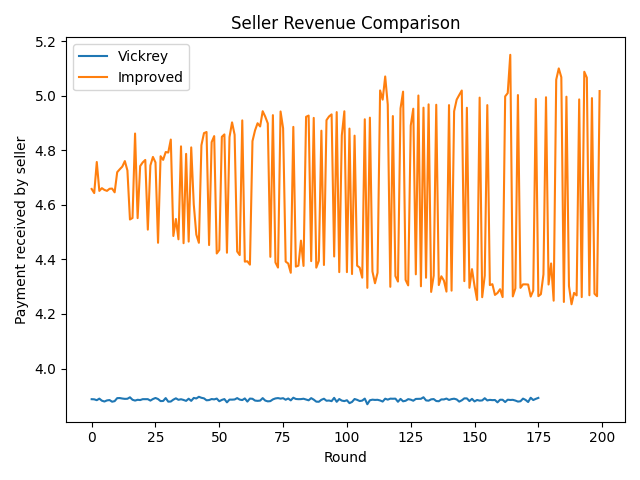
\includegraphics[width=\columnwidth]{../graphs/comparison_payments.png}
\caption{Seller revenue/payment comparison across rounds: Vickrey vs.\ Improved.}
\label{fig:paycomp}
\end{figure}

\begin{figure}[!t]
\centering
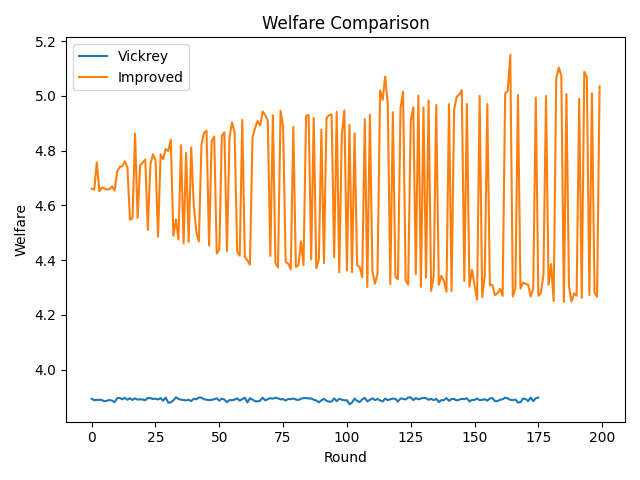
\includegraphics[width=\columnwidth]{../graphs/comparison_welfare.png}
\caption{Welfare proxy comparison across rounds: Vickrey vs.\ Improved.}
\label{fig:welfarecomp}
\end{figure}

\begin{figure}[!t]
\centering
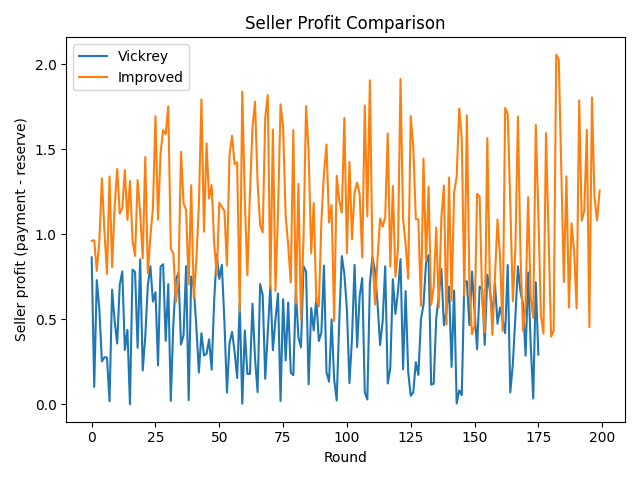
\includegraphics[width=\columnwidth]{../graphs/comparison_seller_profit.png}
\caption{Round-level seller profit comparison: Vickrey vs.\ Improved.}
\label{fig:profitround}
\end{figure}

\begin{figure}[!t]
\centering
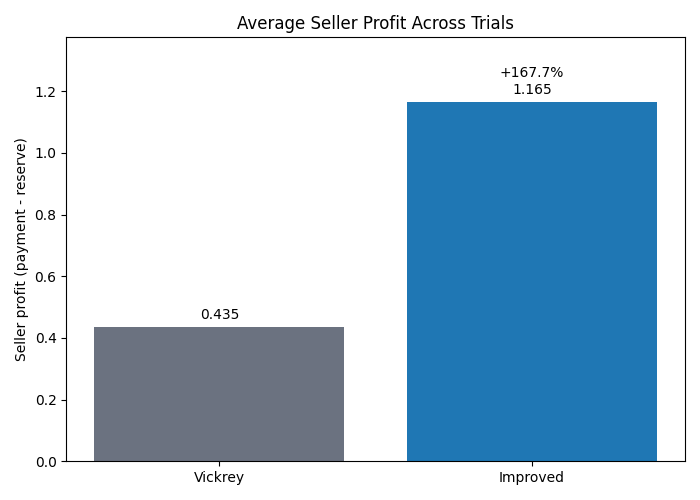
\includegraphics[width=\columnwidth]{../graphs/seller_profit_summary.png}
\caption{Average seller profit across the 20-trial simulation: Vickrey vs.\ Improved.}
\label{fig:sellerprofit}
\end{figure}

\subsection{Graph 1: Payment Comparison Explanation}
Fig.~\ref{fig:paycomp} compares the Vickrey and improved payment received by the seller over auction rounds. The horizontal axis represents the repeated auction round, and the vertical axis represents the second-price payment. The Vickrey curve is almost flat near the reserve-supported clearing level because raw bids are passed directly to the auction. The improved curve stays higher because bid adjustment is applied before clearing. Since both mechanisms still use the same second-price rule, the graph shows that the improved mechanism increases seller revenue by changing the bid environment before settlement, not by replacing the auction rule.

The multi-trial mean confirms the visual pattern. The Vickrey mean payment is $3.8863$, while the improved mean payment is $4.6616$. This is a $19.95\%$ increase in payment. In seller terms, the improved system collects more revenue per cleared auction round under the same simulated collusion conditions.

\subsection{Graph 2: Welfare Comparison Explanation}
Fig.~\ref{fig:welfarecomp} compares the welfare proxy for Vickrey and improved runs. The welfare proxy is the winning cleared bid returned by \texttt{VCGAuction.run}. The improved curve is higher than the Vickrey curve across most rounds. This means the improved mechanism raises the winning-bid proxy used for welfare comparison in the reported simulation.

The aggregate result matches the graph. The Vickrey mean welfare proxy is $3.8909$, while the improved mean welfare proxy is $4.6664$, giving a $19.93\%$ gain. In the code, this metric is the winning cleared bid, and both mechanisms are evaluated with the same welfare definition.

\subsection{Graph 3: Seller Profit Comparison Explanation}
Fig.~\ref{fig:profitround} is the seller-perspective time-series graph. It compares seller profit round by round, where profit is calculated as payment minus reserve floor. This graph is different from the payment graph because reserve floors vary across rounds. A payment can look acceptable but still leave low profit if it is close to the reserve. By subtracting the floor, the graph shows the actual simulated margin above the seller's minimum acceptable value.

The Vickrey curve has lower margin because collusive shading can keep the second-highest valid bid close to reserve. The improved curve is higher and more variable because enforcement strength changes with the detected collusion risk and with bid histories. The reported mean values show that the improved profit level is above the Vickrey method level on average.

\subsection{Graph 4: Average Seller Profit Explanation}
Fig.~\ref{fig:sellerprofit} summarizes the seller-profit result across all 20 trials. This bar chart is included because it gives a direct Vickrey-versus-improved comparison without the noise of individual rounds. The Vickrey average seller profit is $0.4352$, while the improved average seller profit is $1.1649$. The resulting seller-profit gain is $167.68\%$.

The large percentage gain occurs because Vickrey profit above reserve is small. When the Vickrey margin is small, an increase in payment can produce a larger percentage improvement in profit above reserve. In the reported simulation, the improved mechanism gives the seller a larger recorded margin above reserve than the Vickrey method.

\subsection{Combined Explanation from All Graphs}
Taken together, the graphs show a consistent pattern in the generated project outputs. Payment increases, welfare proxy increases, round-level seller profit increases, and average seller profit increases. Here, the improved system raises seller revenue while also raising the implemented winner-bid welfare proxy. The graph set is therefore consistent with the printed result that detection-conditioned bid adjustment improves the reported metrics under the simulated collusive environment.

The graphs also show why the seller-profit metric is included. Payment and welfare graphs show the general upward movement, but the profit graph shows the seller's margin above reserve. Since seller profit is computed directly as payment minus reserve floor, the seller-profit comparison reports the seller-side difference used in the paper.

\FloatBarrier

\section{Seller-Perspective Analysis}
The seller perspective is captured by considering both payment and profit above reserve. Payment shows the absolute revenue collected in the auction. Seller profit, as implemented here, subtracts the reserve floor from that payment. Since the floor represents the seller's minimum acceptable value in the code comment, the profit metric reports the recorded margin above reserve.

In the Vickrey method, the second-price rule can still clear trades, but collusive shading can keep the second-highest valid bid close to the reserve. The seller receives payment, yet the margin above reserve is limited. This is why the Vickrey seller profit mean is only $0.4352$ in the latest run.

In the improved mechanism, the online collusion score controls the enforcement scale passed to the bid adjuster. This adjustment can push bids upward before clearing. Because a second-price auction charges the second-highest valid bid, seller payment increases when adjusted bids raise the second-highest valid bid. This explains why average seller profit rises to $1.1649$ in the reported run.

The seller-profit percentage gain is larger than the payment gain because the Vickrey profit denominator is small. A payment gain of around $20\%$ can translate into a much larger profit-margin gain when the Vickrey method was clearing near reserve. The seller-profit result does not mean total market size increased by $167.68\%$; it means simulated margin above reserve increased by $167.68\%$ under the implemented definition.

\section{Conclusion}
This paper presented the implemented project simulation for comparing the Vickrey method, implemented as a reserve-constrained second-price auction, against an improved collusion-aware auction. The Vickrey method uses raw bids and second-price clearing. The improved mechanism keeps the same second-price clearing rule but adds online collusion scoring and history-aware bid adjustment before the auction is cleared. Both paths are implemented in \texttt{main.py}, which means the reported comparison comes from one executable project script rather than from separate manual calculations.
The latest simulation run uses 1500 generated agents, 200 rounds per trial, and 20 seeded trials. The script loads \texttt{datasets/gpu\_specs\_v7.csv}, filters GPU rows, generates agent values, simulates honest and collusive bidding behavior, clears auctions, stores payment/welfare/seller-profit tuples, evaluates detector metrics, and exports graphs to \texttt{graphs/}. The dataset summary printed by the run reports 3056 source rows, 2823 merged GPU rows, and 2823 missing release-price rows.
The reported aggregate results show that the improved mechanism increases average payment from $3.8863$ to $4.6616$, average welfare proxy from $3.8909$ to $4.6664$, and average seller profit from $0.4352$ to $1.1649$. These correspond to gains of $19.95\%$, $19.93\%$, and $167.68\%$, respectively. The detector evaluation over the improved run reports mean accuracy $0.9000$, ROC-AUC $0.9132$, precision $0.8941$, recall $0.9038$, FPR $0.1019$, and FNR $0.0962$.
These results show that the developed game-theory approach can be used in real-life scenarios. 

\begin{thebibliography}{00}
\bibitem{b1} W. Vickrey, ``Counterspeculation, auctions, and competitive sealed tenders,'' \emph{Journal of Finance}, vol. 16, no. 1, pp. 8--37, 1961.
\bibitem{b2} F. Pedregosa \emph{et al.}, ``Scikit-learn: Machine learning in Python,'' \emph{JMLR}, vol. 12, pp. 2825--2830, 2011.
\bibitem{b3} T. Fawcett, ``An introduction to ROC analysis,'' \emph{Pattern Recognition Letters}, vol. 27, no. 8, pp. 861--874, 2006.
\bibitem{b4} R. B. Myerson, ``Optimal auction design,'' \emph{Mathematics of Operations Research}, vol. 6, no. 1, pp. 58--73, 1981.
\bibitem{b5} P. R. Milgrom and R. J. Weber, ``A theory of auctions and competitive bidding,'' \emph{Econometrica}, vol. 50, no. 5, pp. 1089--1122, 1982.
\bibitem{b6} V. Krishna, \emph{Auction Theory}, 2nd ed. Burlington, MA, USA: Academic Press, 2010.
\bibitem{b7} N. Nisan, T. Roughgarden, E. Tardos, and V. V. Vazirani, Eds., \emph{Algorithmic Game Theory}. Cambridge, U.K.: Cambridge University Press, 2007.
\bibitem{b8} D. Easley and J. Kleinberg, \emph{Networks, Crowds, and Markets: Reasoning About a Highly Connected World}. Cambridge, U.K.: Cambridge University Press, 2010.
\bibitem{b9} L. Breiman, ``Random forests,'' \emph{Machine Learning}, vol. 45, no. 1, pp. 5--32, 2001.
\bibitem{b10} D. W. Hosmer, S. Lemeshow, and R. X. Sturdivant, \emph{Applied Logistic Regression}, 3rd ed. Hoboken, NJ, USA: Wiley, 2013.
\bibitem{b11} R. H. Porter and J. D. Zona, ``Detection of bid rigging in procurement auctions,'' \emph{Journal of Political Economy}, vol. 101, no. 3, pp. 518--538, 1993.
\end{thebibliography}

\end{document}
